\documentclass[conference]{IEEEtran}
\IEEEoverridecommandlockouts
\usepackage[utf8]{inputenc}
\usepackage[T1]{fontenc}
\usepackage{cite}
\usepackage{amsmath,amssymb,amsfonts}
\usepackage{graphicx}
\usepackage{textcomp}
\usepackage{xcolor}
\usepackage{booktabs}
\usepackage{array}
\usepackage{url}
\usepackage[hyphens]{xurl}
\usepackage{balance}

\def\BibTeX{{\rm B\kern-.05em{\sc i\kern-.025em b}\kern-.08em
    T\kern-.1667em\lower.7ex\hbox{E}\kern-.125em X}}

\begin{document}

\title{Local AI Meeting Intelligence Using Parallel LLM\\ Extraction and Hybrid Retrieval}

\author{\IEEEauthorblockN{Sanjay Nesan J}
\IEEEauthorblockA{\textit{Division of Data Science and Cyber Security}\\
\textit{Karunya Institute of Technology and Sciences}\\
Coimbatore, India \\
sanjaynesan@karunya.edu.in}
\and
\IEEEauthorblockN{Dr. Revathi B.S.}
\IEEEauthorblockA{\textit{Division of Data Science and Cyber Security}\\
\textit{Karunya Institute of Technology and Sciences}\\
Coimbatore, India \\
revathi@karunya.edu.in}
}

\maketitle

\begin{abstract}
Meeting recordings hold decisions, action items, risks, and open questions, but sending them to cloud AI services can expose confidential discussions. We built a locally run meeting-intelligence prototype that transcribes and diarizes audio, extracts nine kinds of information in parallel with Qwen2.5-7B, audits each item against the transcript, and answers questions over a stored meeting memory using keyword search, dense retrieval, and Reciprocal Rank Fusion (RRF). On two annotated meetings, extraction reaches a macro F1 of 0.6534; risk extraction is the weakest category (F1 0.250) and its failure modes are analyzed. An audit of 51 stored items flags 3 at the 20\% lexical-overlap threshold; the threshold is shown to be underdetermined on this data, and the check's false-positive and false-negative failure modes are characterized. Over three paired runs, sequential extraction completes all nine stages in $456.3\pm21.1$~s, while parallel runs hit a 300~s client timeout and complete only 17 of 27 stage executions; the 1.49$\times$ speedup is therefore an upper bound, and we trace the failures to Ollama-side queueing rather than slow generation. RAG answers average 11.6~s, 99.4\% of it generation; vector-only retrieval reaches Recall@5 of 0.43, and the implemented hybrid path currently returns a single candidate per query, exposing a fusion defect rather than a benefit. We quantify the privacy--latency trade-off: keeping all content local costs $\sim$456~s of batch extraction and $\sim$12~s of interactive latency on a 4~GB GPU.
\end{abstract}

\begin{IEEEkeywords}
meeting intelligence, speech recognition, large language models, information extraction, hybrid retrieval, transcript grounding, local inference
\end{IEEEkeywords}

\section{Introduction}
Meetings are where organizations make decisions, assign work, and surface risks, yet that knowledge is hard to reuse. Notes miss details, and replaying recordings does not scale as the archive grows. A useful meeting-memory system has to chain several steps: speech recognition, speaker attribution, information extraction, storage, and retrieval. Many meetings also contain confidential material that cannot be sent to third-party cloud services.

This paper describes a prototype built for local processing. Once the models are installed, audio, transcripts, embeddings, and extracted results are handled on the user's own machine, with no external inference API. The pipeline combines speech-to-text and diarization with parallel LLM extraction, schema validation, retries, a transcript-overlap check, incremental embedding, hybrid retrieval, and retrieval-augmented generation (RAG). Commercial assistants such as Microsoft 365 Copilot meeting features \cite{m365}, Zoom AI Companion \cite{zoom}, and Otter.ai \cite{otter} provide this kind of output but process recordings through vendor-hosted models. For organizations whose meetings contain confidential or regulated material, that creates a data-sovereignty gap; an all-local pipeline addresses it. We do not claim quality parity with commercial services, which we did not run; instead we report what the local system achieves on constrained hardware, and document where it currently fails.

We ask three questions. \textbf{RQ1:} How does wall-clock latency compare between sequential and parallel extraction on constrained local hardware, and how many parallel stages complete? \textbf{RQ2:} Does hybrid keyword and dense retrieval beat either method alone? We measure the vector-only baseline and the implemented hybrid path; the hybrid currently degenerates to a single-candidate ranking, so we report the defect and RQ2 stays open. \textbf{RQ3:} How often do extracted items pass the lexical-overlap check, and does that agree with human judgment? We answer the first half, characterize the check's failure modes, and show that its 20\% threshold is not an operating point on our data; human validation is future work.

Our contributions are systems-oriented: (1)~an integrated local pipeline from recording to searchable meeting memory; (2)~a nine-stage parallel extraction design with per-stage validation, whose timing failures we trace to scheduler queueing rather than generation speed; (3)~a retrieval evaluation with a measured vector-only baseline and a documented RRF implementation defect; and (4)~an end-to-end, failure-inclusive evaluation covering extraction quality, a lexical audit, three paired timing runs, a RAG latency profile, and a quantified privacy--latency trade-off. ``Local'' describes the deployment design; we did not verify network isolation.

\section{Related Work}
\textbf{Speech.} Whisper \cite{whisper} provides robust multilingual recognition, WhisperX \cite{whisperx} adds time-aligned long-form transcription, and pyannote.audio \cite{pyannote} identifies who spoke when. These supply the input layer; they do not extract decisions or tasks.

\textbf{Meeting understanding.} QMSum \cite{qmsum} and MeetingBank \cite{meetingbank} are summarization benchmarks, and the AutoMin shared task \cite{automin} studied automatic minuting. Structured-output methods \cite{structured} help downstream processing, but independent extraction of several categories still needs validation against the source transcript.

\textbf{Commercial meeting assistants.} The commercial systems named in Sec.~I transcribe and summarize meetings in vendor clouds. The gap we target is deployment location, not feature coverage: keeping recordings, transcripts, and extracted outputs on the user's own machine. Quality comparisons against those products are outside this study; we provide the local reference instead.

\textbf{Retrieval.} RAG \cite{rag} grounds generation in retrieved text, and dense retrieval \cite{dpr} complements lexical methods such as BM25 \cite{bm25}. Our MongoDB keyword path is a weighted field-match score, not BM25. RRF \cite{rrf} merges ranked lists without calibrating their scores.

\textbf{Hallucination.} LLM output can include unsupported statements \cite{halluc}. SelfCheckGPT \cite{selfcheck} is one detector; we do not use it. Our word-overlap check is a cheap audit signal and cannot establish entailment.

\textbf{Gap.} Each component is well studied. Our contribution is their integration into one local meeting-memory workflow, plus an end-to-end measurement that includes failures. We claim no new model or retrieval algorithm.

\section{System Design}
\subsection{Architecture}
Fig.~\ref{fig:arch} shows the pipeline. Audio or video is transcribed and diarized, the speaker-attributed transcript goes to a parallel extraction layer, outputs are validated and normalized, and results are indexed for keyword and semantic search. At query time, keyword and vector rankings are fused with RRF and passed to the RAG component. A React front end and a Node.js/Express backend coordinate the services.

\begin{figure*}[t]
\centering
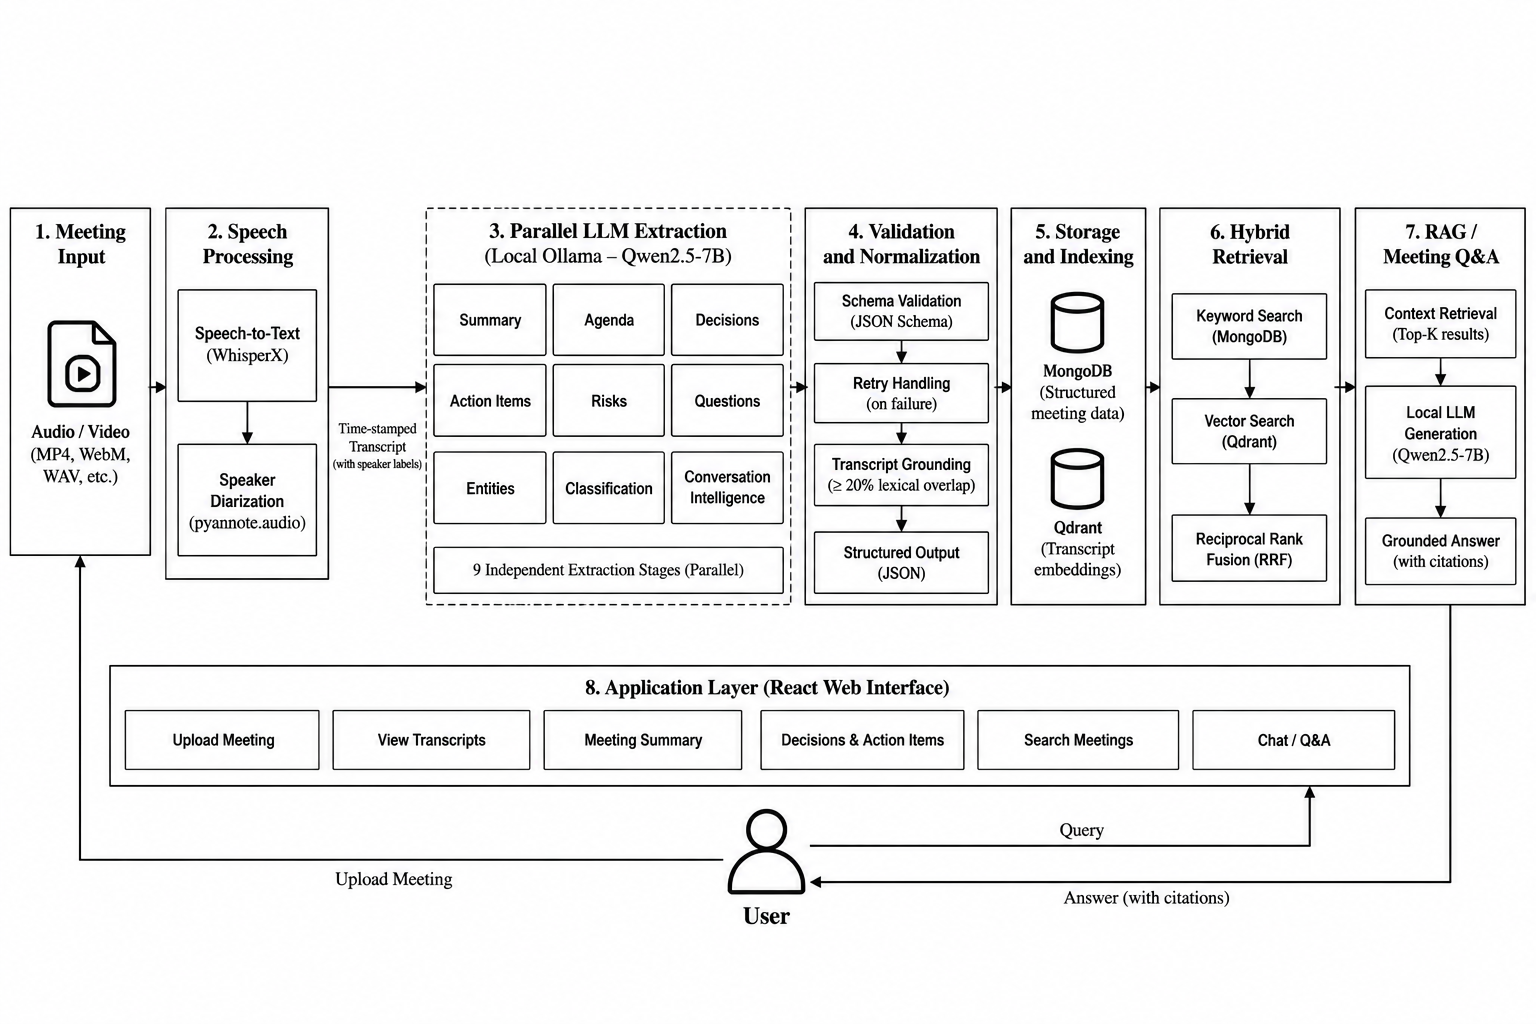
\includegraphics[width=0.78\textwidth]{../figs/fig1_architecture}
\caption{Architecture of the local meeting-intelligence pipeline: (1)~meeting input, (2)~speech-to-text and diarization producing a time-stamped, speaker-labeled transcript, (3)~nine parallel LLM extraction stages, (4)~schema validation, retry, and $\geq$20\% transcript grounding, (5)~MongoDB/Qdrant indexing, (6)~hybrid retrieval with RRF, and (7)~RAG question answering with citations; (8)~the React application layer connects the user.}
\label{fig:arch}
\end{figure*}

\subsection{Speech Processing}
A CTranslate2-based Whisper model produces a time-aligned transcript, and pyannote.audio runs diarization separately. Each transcript segment is assigned to the diarization segment it overlaps most, so every statement carries a speaker label. This matters because decisions and action items are usually tied to a person.

\subsection{Parallel Extraction}
Instead of one large prompt, the system runs nine independent stages with the local LLM: (1)~summary, (2)~agenda, (3)~decisions, (4)~action items, (5)~risks, (6)~questions, (7)~entities, (8)~meeting classification, and (9)~conversational intelligence. Each stage has its own prompt, output schema, and retry handling, so one failed stage does not block the others. Outputs are schema-checked and normalized (for example, priorities and deadlines) before storage.

\subsection{Transcript Grounding}
\label{sec:design:grounding}
For selected fields, we take each item's words longer than three characters and check how many occur in the source transcript. An item passes if at least 20\% do. The threshold was set as an operating point for flagging nearly unsupported content; it has not been calibrated against human judgments. The check compares against the whole transcript, so broadly on-topic text can pass, and it says nothing about meaning. Two failure modes bound any lexical check: a supported but paraphrased item can be \emph{flagged} because its words do not recur (false positive), and an unsupported but on-topic statement can \emph{pass} because shared topic vocabulary overlaps without entailment (false negative). Behavior on failure differs by field: most validators log the failure and keep the item, while risk validation can drop it.

\subsection{Indexing and Hybrid Retrieval}
Transcripts are split into chunks of up to 500 characters, each with a deterministic ID and content hash so unchanged chunks are skipped on re-indexing. Embeddings from \texttt{nomic-embed-text} go to Qdrant; structured results and metadata go to MongoDB. For a query, RRF fuses the two ranked lists:
\begin{equation}
\mathrm{RRF}(d)=\sum_{i=1}^{m}\frac{1}{k+\mathrm{rank}_i(d)},\qquad k=60,
\label{eq:rrf}
\end{equation}
where $m$ is the number of lists and an item missing from a list adds no term. MongoDB ranking is an additive field-weight score: each case-insensitive match adds the field's weight (decisions 10, action items 9, summaries and keywords 8, transcript 3). MongoDB ranks whole meetings while Qdrant returns chunks, so the implementation fuses by meeting ID when available. The fused context goes to the local LLM, which answers from the retrieved material.

\subsection{Application Interface}
Fig.~\ref{fig:ui} shows the web application: (a)~an organization analytics view with trend, sentiment, and engagement charts, (b)~a meeting-memory chat that answers questions with cited source meetings, (c)~a per-meeting AI dashboard reporting extracted counts and a health score, and (d)~a meeting detail view with action items, entities, and answered and unanswered questions.

\begin{figure*}[t]
\centering
\begin{minipage}[t]{0.49\textwidth}\centering
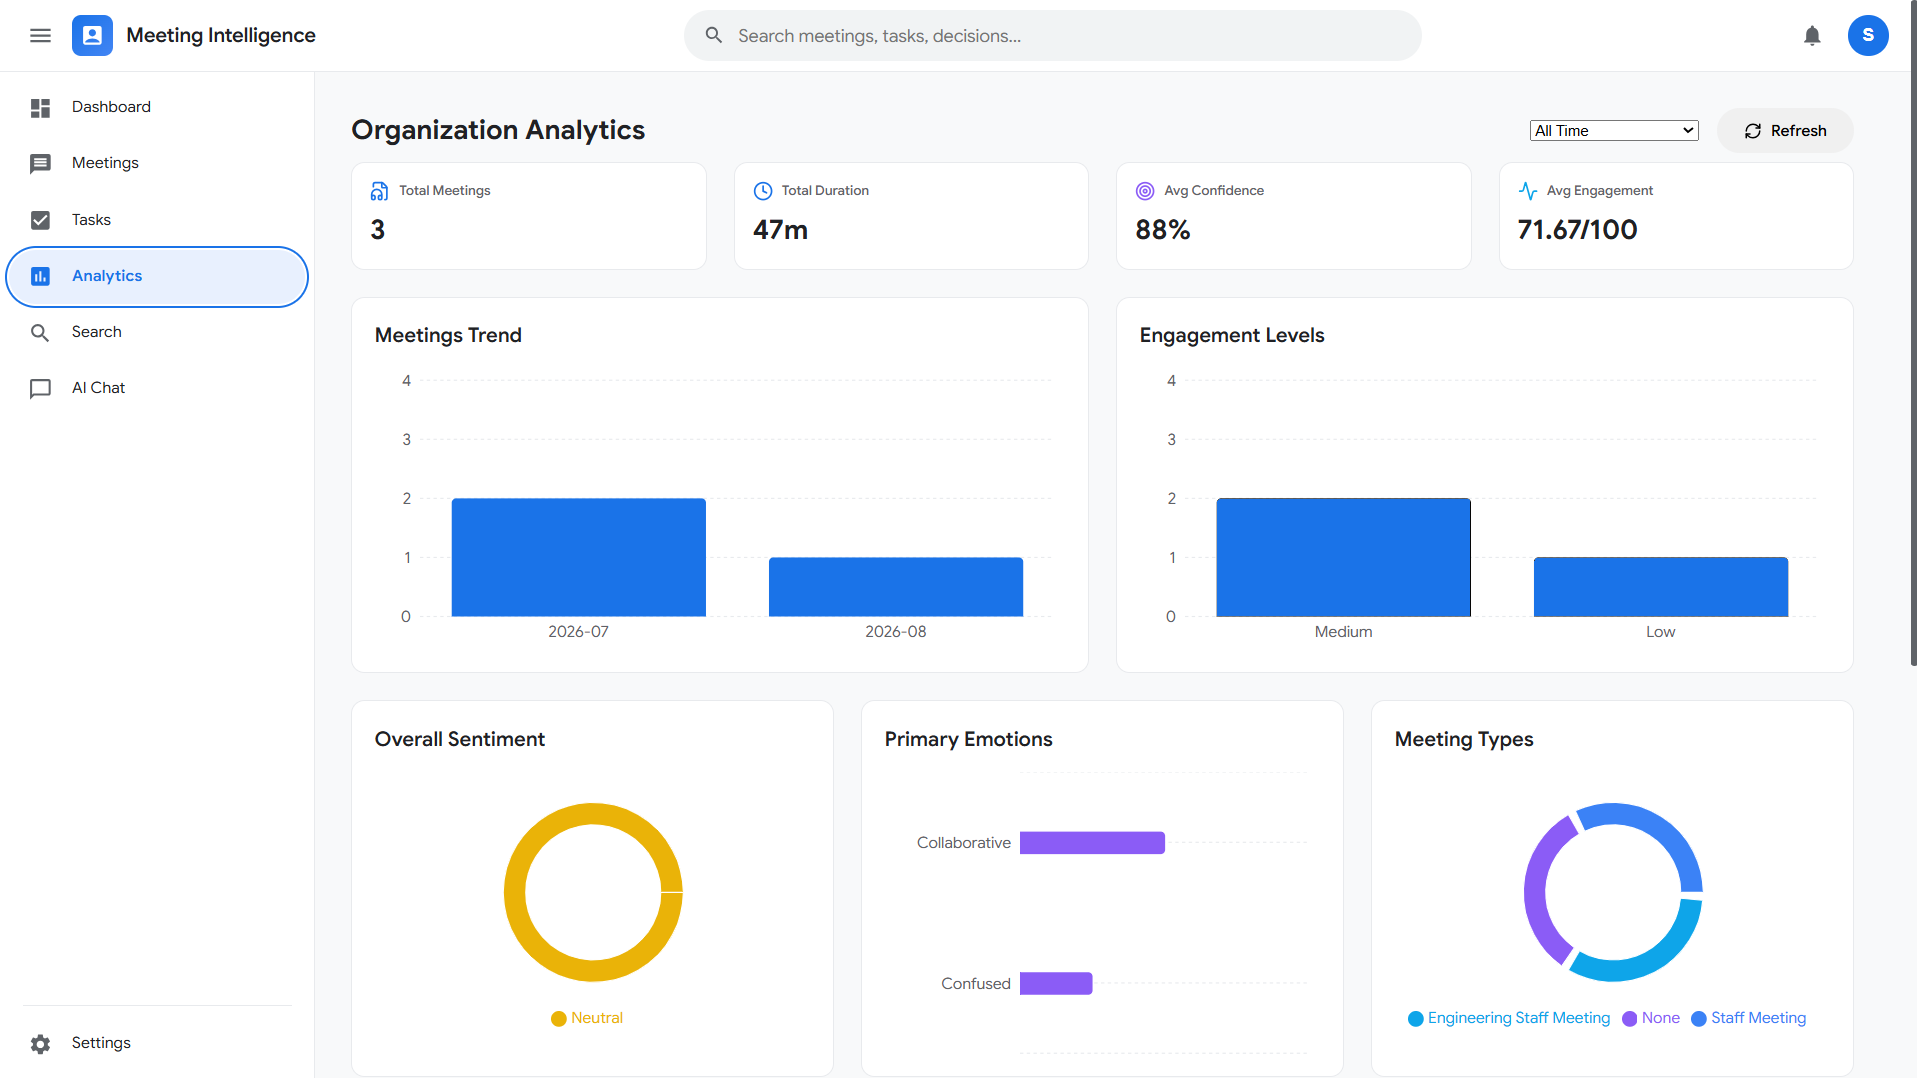
\includegraphics[width=\linewidth]{../figs/fig2_org_analytics}\\[1pt]{\footnotesize (a) Organization analytics}
\end{minipage}\hfill
\begin{minipage}[t]{0.49\textwidth}\centering
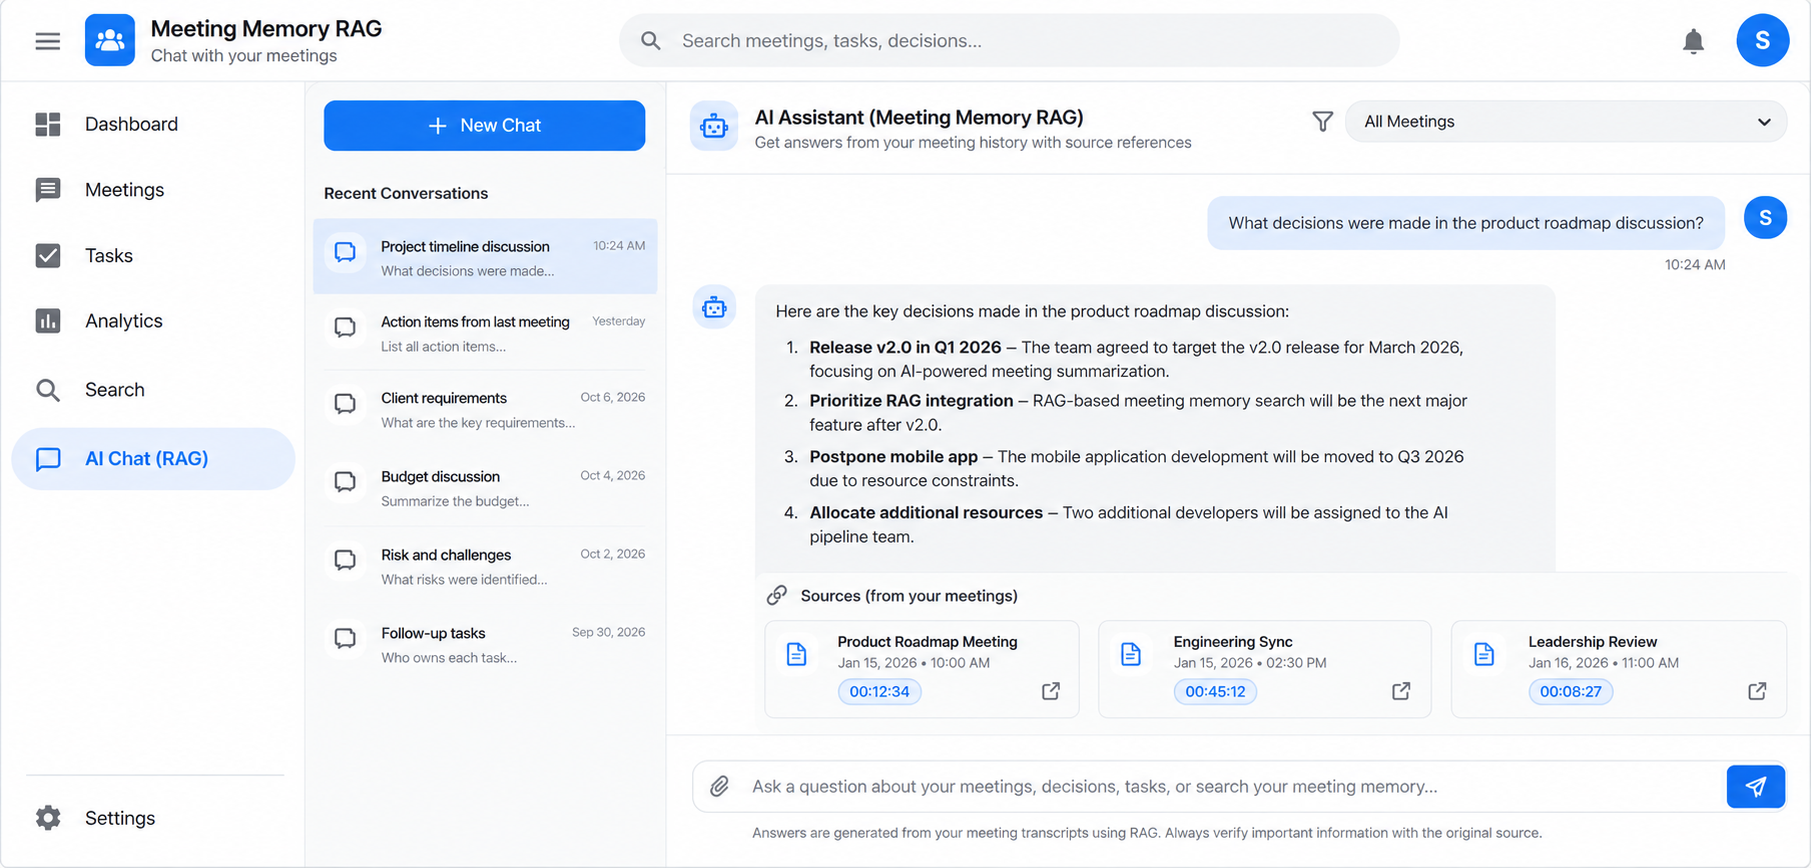
\includegraphics[width=\linewidth]{../figs/fig3_rag_interface}\\[1pt]{\footnotesize (b) Meeting-memory Q\&A}
\end{minipage}

\begin{minipage}[t]{0.49\textwidth}\centering
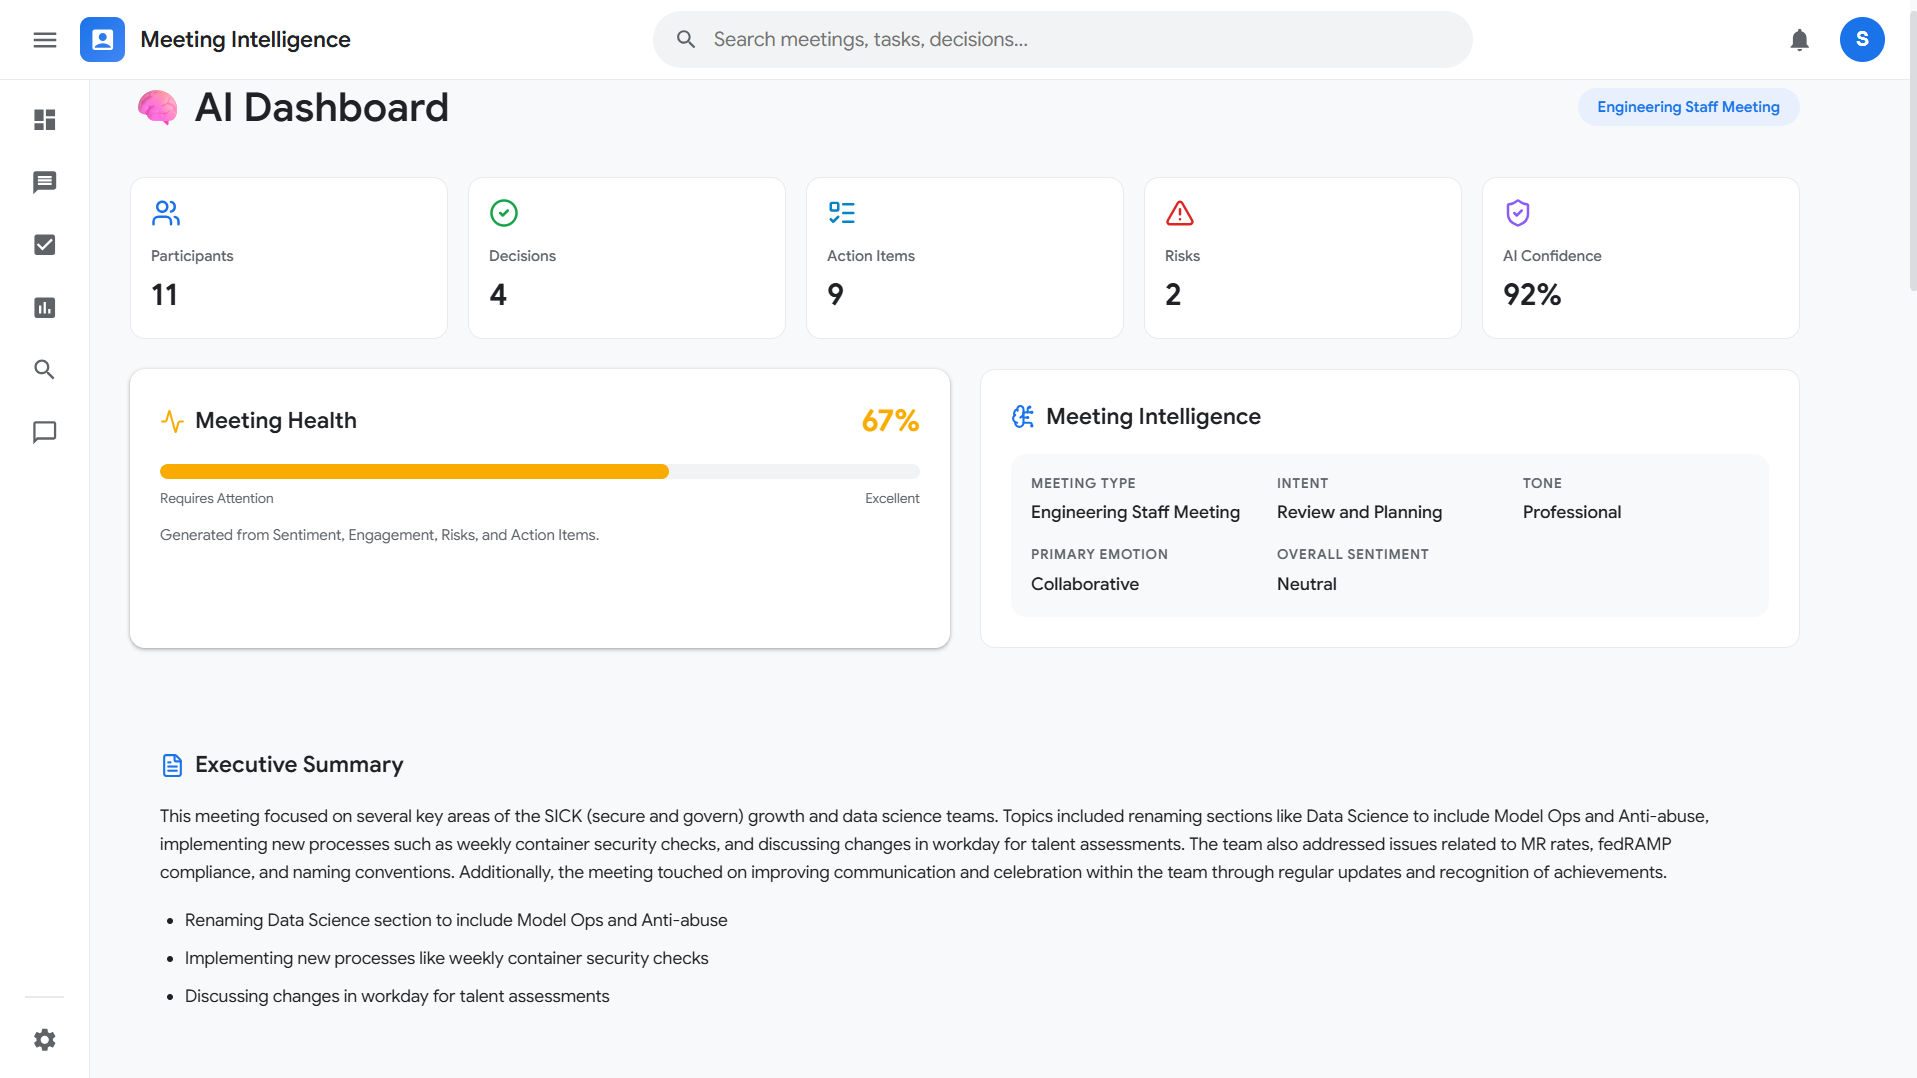
\includegraphics[width=\linewidth]{../figs/fig4_meeting_dashboard}\\[1pt]{\footnotesize (c) Meeting AI dashboard}
\end{minipage}\hfill
\begin{minipage}[t]{0.49\textwidth}\centering
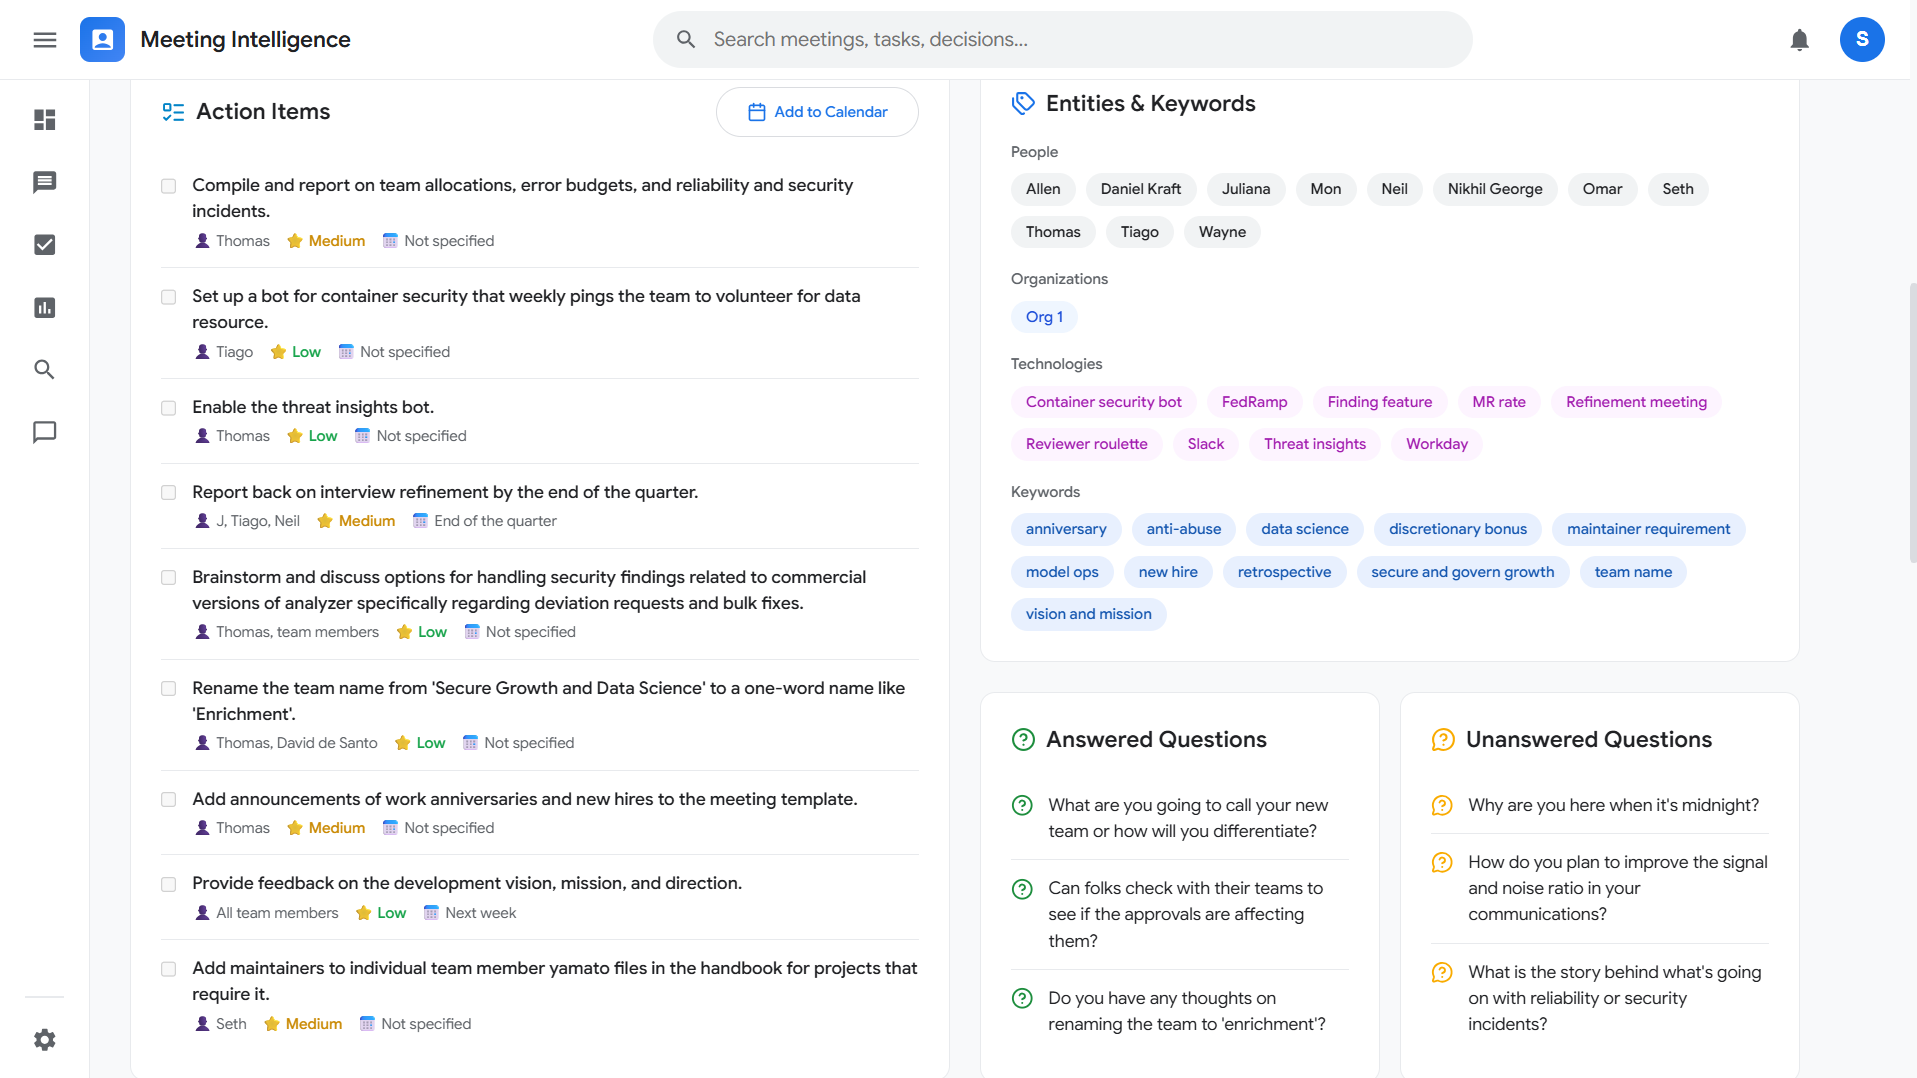
\includegraphics[width=\linewidth]{../figs/fig5_meeting_detail}\\[1pt]{\footnotesize (d) Meeting detail}
\end{minipage}
\caption{Application interface: (a)~organization-level analytics with trend and sentiment charts, (b)~meeting-memory question answering with cited source meetings, (c)~per-meeting AI dashboard with extracted counts and health score, and (d)~meeting detail with action items, entities, and question panels.}
\label{fig:ui}
\end{figure*}

\section{Experimental Methodology}
\subsection{Setup}
We used Ollama with \texttt{qwen2.5:7b} \cite{qwen} (Q4\_K\_M, 7.6B parameters), temperature 0, an 8,192-token context, and a 24,000-character transcript limit. The workstation ran Windows 11 (Node.js v22.14.0, CUDA 12.8, Python 3.10) on a Core i5-12450H CPU with 16~GB RAM and an RTX 3050 Laptop GPU with 4,096~MiB. Embeddings used Nomic Embed \cite{nomic} at 768 dimensions. The run configuration recorded \texttt{OLLAMA\_NUM\_PARALLEL=4}, \texttt{OLLAMA\_MAX\_LOADED\_MODELS=1}, and a 360,000~ms request timeout.

The model file is about 4.7~GB, so it cannot fit in 4~GB of VRAM. Profiling showed a peak of 3,431~MiB in use with 532~MiB free, so part of the model runs from host memory (the layer split was not reported). Free host RAM was low (about 0.4--1.6~GB), and one load attempt was refused for lack of memory.

The timing runs used a 24,015-character input that the log identifies as the largest stored transcript. We map it to Sec Growth DataScience (24,310 characters), so about 1.2\% of that transcript was left out; the log does not store the transcript ID, so this mapping is inferred.

\subsection{Corpus}
The system holds three meetings (47.64 min, 7,987 words; Table~\ref{tab:corpus}). Extraction is scored on two of them, ``Effective Meetings'' and ``SICK -- Secure and Govern Growth'' (7,245 words, 2,593.08~s). The Tamil-labeled recording is excluded because its spoken language is unverified (its language field says English). The lexical audit covers all three. Speaker counts, domains, and acoustic conditions were not recorded.

\begin{table}[!t]
\caption{Meeting Inventory (NR: not recorded)}
\label{tab:corpus}
\centering
\footnotesize
\setlength{\tabcolsep}{3pt}
\begin{tabular}{lrrcccc}
\toprule
\textbf{ID} & \textbf{Dur. (s)} & \textbf{Words} & \textbf{Spk.} & \textbf{Domain} & \textbf{Lang.} & \textbf{Acoust.}\\
\midrule
Tamil audio$^{*}$ & 265.31 & 742 & NR & NR & en & NR\\
Sec Growth & 1,743.47 & 4,647 & NR & NR & en & NR\\
Effective Meetings & 849.61 & 2,598 & NR & NR & en & NR\\
\bottomrule
\multicolumn{7}{l}{\scriptsize $^{*}$Title says Tamil; stored language field is English.}
\end{tabular}
\end{table}

\subsection{Metrics and Benchmarks}
\emph{Extraction.} The two reference files contain 37 manual annotations; annotator count and guidelines were not documented. Predictions are greedily matched one-to-one to the unused reference with the highest token Jaccard similarity (threshold 0.5), which can penalize paraphrases. We compute precision, recall, and F1 per category from counts pooled over both meetings and macro-average F1 over the four categories.

\emph{Timing.} Three paired runs each processed the same transcript sequentially (nine stages in turn) and in parallel (nine concurrent requests), logging per-stage time, status, and error cause.

\emph{RAG latency.} Five questions $\times$ three runs (N=15), with Qdrant available, top-K of 10, a 10,000-character context limit, and temperature 0.3, with separate timers for embedding, Qdrant search, retrieval, and generation.

\emph{Retrieval quality.} Keyword (MongoDB), vector (Qdrant), and RRF rankings were scored on the same 35 chunk-level labeled queries at $k\in\{1,3,5,10\}$; the labeling procedure was not documented, which we report as a limitation. Sec.~\ref{sec:retrieval} explains why the keyword scores are not meaningful at chunk level.

\section{Results and Discussion}
\subsection{Extraction}
Table~\ref{tab:extraction} shows macro F1 of 0.6534 over 37 reference items and 34 predictions. Unanswered questions were extracted perfectly on this small set, action items reached F1 0.727, and decisions 0.636.

Risks were the weakest category (F1 0.250: one of four found, three false positives). The false positives are fabricated risks with no explicit transcript support, which is the same class of error the grounding audit later flags (Sec.~\ref{sec:grounding}). With only four reference risks, each hit moves the F1 by 0.25, so this category score is not stable. Because risks are rarely stated explicitly in meetings, we attribute part of the weakness to the prompt: the drafted revision requires each risk to carry a verbatim evidence quote (Sec.~\ref{sec:limits}), which also strengthens grounding. On two meetings, all of these numbers are preliminary.

\begin{table}[!t]
\caption{Extraction Results on Two Annotated Meetings}
\label{tab:extraction}
\centering
\footnotesize
\setlength{\tabcolsep}{3.4pt}
\renewcommand{\arraystretch}{1.05}
\begin{tabular}{lrrrrrrrr}
\toprule
\textbf{Category} & \textbf{Ref} & \textbf{Pred} & \textbf{TP} & \textbf{FP} & \textbf{FN} & \textbf{P} & \textbf{R} & \textbf{F1}\\
\midrule
Decisions & 12 & 10 & 7 & 3 & 5 & 0.7000 & 0.5833 & 0.6364\\
Action items & 17 & 16 & 12 & 4 & 5 & 0.7500 & 0.7059 & 0.7273\\
Risks & 4 & 4 & 1 & 3 & 3 & 0.2500 & 0.2500 & 0.2500\\
Unanswered q. & 4 & 4 & 4 & 0 & 0 & 1.0000 & 1.0000 & 1.0000\\
\midrule
Macro average & -- & -- & -- & -- & -- & 0.6750 & 0.6348 & 0.6534\\
\bottomrule
\end{tabular}
\end{table}

\subsection{Grounding}
\label{sec:grounding}
Of 51 stored items from all three meetings, 48 passed the 20\% check and 3 were flagged (5.88\%; Table~\ref{tab:grounding}). Two of the four risks were flagged, in line with the weak risk F1. The three flagged items have zero overlap, so thresholds from 10\% to 50\% all flag the same 3 of 51; on this data the sweep cannot choose a threshold, and the 20\% value remains a design choice, not a calibrated operating point. The two failure modes described in Sec.~\ref{sec:design:grounding} therefore bound the check: it will both flag valid paraphrases and miss lexically plausible hallucinations. The unanswered-question count here (12) covers three meetings and differs from the two-meeting count in Table~\ref{tab:extraction} (4). The audit rescores saved database items without replaying the current validator, so it cannot say whether today's pipeline would keep the flagged risks. Passing the check is not evidence of accuracy.

\begin{table}[!t]
\caption{Saved-Output Grounding Audit by Category}
\label{tab:grounding}
\centering
\footnotesize
\begin{tabular}{lrrrr}
\toprule
\textbf{Category} & \textbf{Total} & \textbf{Pass} & \textbf{Flagged} & \textbf{Flag rate}\\
\midrule
Decisions & 10 & 10 & 0 & 0.00\%\\
Action items & 17 & 17 & 0 & 0.00\%\\
Risks & 4 & 2 & 2 & 50.00\%\\
Answered questions & 8 & 8 & 0 & 0.00\%\\
Unanswered questions & 12 & 11 & 1 & 8.33\%\\
\midrule
Aggregate & 51 & 48 & 3 & 5.88\%\\
\bottomrule
\end{tabular}
\end{table}

\subsection{Sequential versus Parallel Extraction (RQ1)}
\label{sec:proc}
Table~\ref{tab:timing} gives the three paired runs. Sequential extraction completed all nine stages every time ($456{,}318\pm21{,}081$~ms). In every parallel run, two to five stages failed with \texttt{fetch failed}, each with the cause \texttt{UND\_ERR\_HEADERS\_TIMEOUT}, and only 17 of 27 stage executions completed. All parallel runs ended at 306.5--306.7~s, which is 300~s plus a few seconds. That matches Node's default 300~s headers timeout, not our configured 360~s, and it means queued requests waited at least 300~s for Ollama to respond. An earlier single run showed the same pattern (490,289 versus 306,385~ms with four failed stages; the 37.51\% reduction quoted from that run is one instance of the same ceiling).

Failed stages would have needed more than 306.5~s, so a complete parallel run takes at least that long. The parallel mean is therefore a timeout ceiling, and 1.49$\times$ (a 32.8\% reduction) is an upper bound, not a measured speedup.

\emph{Concurrency and contention.} Three observations tie the failures to the configuration. First, \texttt{OLLAMA\_MAX\_LOADED\_MODELS=1} plus a 4.7~GB model that is only partially in VRAM (3,431~MiB used; free host RAM 0.4--1.6~GB) throttles the shared throughput. Second, the failed requests include risk extraction, which finishes in 8.5~s sequentially; its parallel failure is therefore a request queued behind 300~s of scheduler waiting, not slow generation. Third, action items took 270.8~s in parallel run~1 versus 142.6~s sequentially, consistent with slot contention under \texttt{OLLAMA\_NUM\_PARALLEL=4}. The implication is that sequential execution is the reliable mode on this hardware (9/9 complete in all three runs); parallelism pays only when the concurrency is capped to the number of Ollama slots and the client timeout is raised (the client was patched to 900~s; the rerun is scheduled). On the hardware side, $\ge$8~GB VRAM so the model stays resident, or a 3B-class model for extraction, would shrink both modes; a single-prompt baseline is the natural lower-cost alternative to compare against.

\begin{table}[!t]
\caption{Paired Sequential and Parallel Extraction Timing}
\label{tab:timing}
\centering
\footnotesize
\setlength{\tabcolsep}{2.2pt}
\begin{tabular}{lrrcc}
\toprule
\textbf{Run} & \textbf{Seq. (ms)} & \textbf{Par. (ms)} & \textbf{Par. OK} & \textbf{Speedup$^{\dagger}$}\\
\midrule
1 & 478,409 & 306,712 & 4/9 & 1.56\\
2 & 454,127 & 306,537 & 6/9 & 1.48\\
3 & 436,419 & 306,497 & 7/9 & 1.42\\
\midrule
Mean$\pm$std & 456,318$\pm$21,081 & 306,582$\pm$114 & 17/27 & 1.49$\pm$0.07\\
\bottomrule
\multicolumn{5}{p{0.93\columnwidth}}{\scriptsize $^{\dagger}$Upper bound: failed parallel stages were cut off at the timeout.}
\end{tabular}
\end{table}

\subsection{RAG Latency}
Table~\ref{tab:rag} breaks down the RAG path with Qdrant active. Qdrant search takes 37.4~ms, but query embedding takes about 2.7~s in 14 of 15 runs and generation about 11.5~s, which is 99.4\% of end-to-end time. The first run's embedding took 105~ms; every later run took 2.7--3.0~s. Because only one model may stay loaded, the embedding and generation models may be evicting each other, which we have not yet tested. The retrieval timer was shorter than the embedding timer in all 15 runs, so the two are not additive and we report them separately. Every query also retrieved only one chunk (472--496 characters) although Qdrant returned eight hits, and one answer was empty, so context assembly needs debugging. Answer quality was not evaluated. Mitigations (keeping both models resident, embedding caches, a smaller answer model, precomputation) are discussed in Sec.~\ref{sec:tradeoff}; none is measured here.

\begin{table}[!t]
\caption{RAG Latency with Qdrant Active (N=15)}
\label{tab:rag}
\centering
\footnotesize
\begin{tabular}{lcc}
\toprule
\textbf{Component} & \textbf{Mean $\pm$ std (ms)} & \textbf{Range (ms)}\\
\midrule
Query embedding & 2,669.1 $\pm$ 714.8 & 105--2,998\\
Qdrant ANN search & 37.4 $\pm$ 13.7 & 14--62\\
Retrieval timer & 73.4 $\pm$ 12.6 & 59--98\\
Generation & 11,512.2 $\pm$ 1,171.8 & 10,487--15,483\\
End to end & 11,585.6 $\pm$ 1,179.6 & 10,551--15,581\\
\bottomrule
\end{tabular}
\end{table}

\subsection{Retrieval Quality (RQ2)}
\label{sec:retrieval}
Table~\ref{tab:retrieval} compares the three ranking paths on the same 35 labeled queries. The vector-only baseline is interpretable: the relevant chunk is in the top five for 42.9\% of queries and the top ten for 68.6\%, but first for only 8.6\%, so dense search finds relevant chunks but ranks them poorly. The hybrid path scored 0.0857 at every cutoff, equal to vector Recall@1: the fused ranking returned at most one candidate per query, so Recall@$k$ and nDCG@$k$ collapse to their $k{=}1$ value at all cutoffs. This matches the single retrieved chunk in the RAG logs and points to a fusion defect, not to ``hybrid is no better.'' The keyword path scored zero at every cutoff, but MongoDB ranks whole meetings while the labels are chunk IDs; a zero is expected from the granularity mismatch and says nothing about keyword quality. The logged MRR (0.0857) and precision values are inconsistent with the recall numbers (three rank-one hits plus twelve more in the top five imply MRR of at least 0.154), so we withhold them. Until the fusion path returns full chunk rankings, RQ2 remains open.

\begin{table}[!t]
\caption{Retrieval Quality, 35 Labeled Chunk Queries}
\label{tab:retrieval}
\centering
\footnotesize
\setlength{\tabcolsep}{3pt}
\begin{tabular}{lcccc}
\toprule
\textbf{Path} & \textbf{R@$1$} & \textbf{R@$3$} & \textbf{R@$5$} & \textbf{R@$10$}\\
\midrule
Vector-only (Qdrant) & 0.0857 & 0.2571 & 0.4286 & 0.6857\\
RRF hybrid (current) & 0.0857 & 0.0857 & 0.0857 & 0.0857$^{*}$\\
Keyword (MongoDB) & n/m & n/m & n/m & n/m$^{\dagger}$\\
\midrule
\multicolumn{5}{l}{\scriptsize Vector nDCG@1/3/5/10: 0.0857 / 0.1827 / 0.2527 / 0.3389.}\\
\multicolumn{5}{l}{\scriptsize $^{*}$Degenerate: fused ranking returned $\le$1 candidate per query.}\\
\multicolumn{5}{l}{\scriptsize $^{\dagger}$n/m = not meaningful: meeting-level rankings vs. chunk labels.}\\
\bottomrule
\end{tabular}
\end{table}

\subsection{Privacy--Latency Trade-off}
\label{sec:tradeoff}
Local deployment buys data locality at a measurable latency cost. The current measurements are: one $\sim$24,000-character transcript produces nine structured outputs in about 456~s sequentially, and an interactive answer takes about 12~s end to end, of which 99.4\% is 7B-model generation and $\sim$2.7~s is embedding (amplified by model eviction under \texttt{OLLAMA\_MAX\_LOADED\_MODELS=1}). On a 4~GB GPU this system is therefore slower than typical cloud assistants, which is the price of keeping every byte on the machine; we have not run a network-isolation test, so ``local'' is a design property, not a verified guarantee. The latency profile suggests concrete levers, none measured here: keep both models resident to remove the embedding penalty, cache query embeddings, precompute context, or answer with a 3B-class model while reserving the 7B model for batch extraction. The trade-off is explicit: minute-scale batch and $\sim$12~s interactive responses in exchange for no off-machine data flow.

\section{Limitations and Future Work}
\label{sec:limits}
The evaluation is small and early. Extraction uses two annotated meetings with undocumented annotation and a strict matching rule. The overlap check compares against the full transcript, has characterized false-positive and false-negative modes, no human validation, and a threshold that the data cannot calibrate. The parallel timing has no valid completion time because of the client timeout. Retrieval quality is measured only for vector search; the hybrid path is defective (single-candidate rankings) and the keyword baseline is incommensurate at chunk level. Labels for the 35 queries lack documented procedure. The 7B model runs in a CPU/GPU split with little free host RAM, which limits throughput and reproducibility. Long transcripts are truncated at 24,000 characters, and the Tamil-labeled recording is unverified. We ran no network-isolation test, so we use ``local'' and not ``privacy-preserving.''

Next steps, in order: (1)~rerun the paired timing with the patched 900~s client, concurrency capped to Ollama slots, \texttt{OLLAMA\_NUM\_PARALLEL} set on the \texttt{ollama serve} process, and per-stage attempt logging; (2)~repair retrieval evaluation by returning ranked chunks from fusion, adding a chunk-level keyword baseline, recomputing MRR and precision, documenting the query labels, and confirming Nomic's recommended task prefixes; (3)~test keeping both models resident to remove the embedding delay. Further work includes a single-prompt baseline, a 10--15 meeting corpus across meeting types, lengths, and acoustic conditions (with AMI \cite{ami} as a public option), two-annotator grounding judgments with Cohen's $\kappa$, a local NLI check in place of lexical overlap, sliding-window grounding, a risk prompt that requires verbatim evidence quotes, and a quality comparison against commercial assistants on a common labeled set once the retrieval path is repaired. An egress-monitored privacy test would upgrade ``local'' to a verified property.

\section{Conclusion}
We presented a local pipeline that turns meeting recordings into searchable, structured memory. Extraction reaches a macro F1 of 0.6534 on two meetings, with risk extraction identified and analyzed as the weak point. Sequential extraction runs reliably in about 456~s; on a 4~GB GPU, parallel extraction was cut short by a 300~s client timeout, so only an upper-bound speedup of 1.49$\times$ is established, and we traced the failures to scheduler queueing rather than generation speed. Vector-only retrieval reaches Recall@5 of 0.43; the hybrid path currently degenerates to a single-candidate ranking, and keyword scores are not comparable at chunk level. The privacy--latency trade-off is quantified: $\sim$456~s batch extraction and $\sim$12~s interactive answers, all local. What remains open is a completed parallel speedup, demonstrated hybrid benefit, human-validated grounding, and verified network isolation, and the planned fixes target exactly those gaps.

\balance
\begin{thebibliography}{00}
\bibitem{whisper} A. Radford, J. W. Kim, T. Xu, G. Brockman, C. McLeavey, and I. Sutskever, ``Robust speech recognition via large-scale weak supervision,'' in \textit{Proc. 40th Int. Conf. Machine Learning (ICML)}, PMLR vol. 202, 2023, pp. 28492--28518.
\bibitem{whisperx} M. Bain, J. Huh, T. Han, and A. Zisserman, ``WhisperX: Time-accurate speech transcription of long-form audio,'' in \textit{Proc. INTERSPEECH}, 2023, pp. 4489--4493.
\bibitem{pyannote} H. Bredin, ``pyannote.audio 2.1 speaker diarization pipeline: Principle, benchmark, and recipe,'' in \textit{Proc. INTERSPEECH}, 2023, pp. 1983--1987, doi: 10.21437/Interspeech.2023-105.
\bibitem{qmsum} M. Zhong \textit{et al.}, ``QMSum: A new benchmark for query-based multi-domain meeting summarization,'' in \textit{Proc. NAACL-HLT}, 2021, pp. 5905--5921.
\bibitem{meetingbank} Y. Hu \textit{et al.}, ``MeetingBank: A benchmark dataset for meeting summarization,'' in \textit{Proc. 61st Annu. Meeting Assoc. Comput. Linguistics}, vol. 1: Long Papers, 2023, pp. 16409--16423.
\bibitem{automin} T. Ghosal, O. Bojar, M. Hled\'{\i}kov\'{a}, T. Kocmi, and A. Nedoluzhko, ``Overview of the first shared task on automatic minuting (AutoMin) at INTERSPEECH 2021,'' in \textit{Proc. First Shared Task on Automatic Minuting at INTERSPEECH 2021}, 2021, pp. 1--25.
\bibitem{structured} S. Geng \textit{et al.}, ``Generating structured outputs from language models: Benchmark and studies,'' arXiv:2501.10868, 2025.
\bibitem{rag} P. Lewis \textit{et al.}, ``Retrieval-augmented generation for knowledge-intensive NLP tasks,'' in \textit{Advances in Neural Information Processing Systems (NeurIPS)}, vol. 33, 2020, pp. 9459--9474.
\bibitem{dpr} V. Karpukhin \textit{et al.}, ``Dense passage retrieval for open-domain question answering,'' in \textit{Proc. 2020 Conf. Empirical Methods in Natural Language Processing (EMNLP)}, 2020, pp. 6769--6781.
\bibitem{bm25} S. Robertson and H. Zaragoza, ``The probabilistic relevance framework: BM25 and beyond,'' \textit{Foundations and Trends in Information Retrieval}, vol. 3, no. 4, pp. 333--389, 2009.
\bibitem{rrf} G. V. Cormack, C. L. A. Clarke, and S. Buettcher, ``Reciprocal rank fusion outperforms Condorcet and individual rank learning methods,'' in \textit{Proc. 32nd Int. ACM SIGIR Conf. Research and Development in Information Retrieval}, 2009, pp. 758--759.
\bibitem{halluc} L. Huang \textit{et al.}, ``A survey on hallucination in large language models: Principles, taxonomy, challenges, and open questions,'' \textit{ACM Trans. Information Systems}, 2024, arXiv:2311.05232.
\bibitem{selfcheck} P. Manakul, A. Liusie, and M. Gales, ``SelfCheckGPT: Zero-resource black-box hallucination detection for generative large language models,'' in \textit{Proc. EMNLP}, 2023, pp. 9004--9017.
\bibitem{qwen} A. Yang \textit{et al.}, ``Qwen2.5 technical report,'' arXiv:2412.15115, 2024.
\bibitem{nomic} Z. Nussbaum, J. X. Morris, B. Duderstadt, and A. Mulyar, ``Nomic embed: Training a reproducible long context text embedder,'' arXiv:2402.01613, 2024.
\bibitem{ami} J. Carletta \textit{et al.}, ``The AMI meeting corpus: A pre-announcement,'' in \textit{Machine Learning for Multimodal Interaction}, 2006, pp. 28--39.
\bibitem{m365} Microsoft, ``Microsoft 365 Copilot meeting features,'' Microsoft Learn, 2024. [Online]. Available: \url{https://learn.microsoft.com/microsoft-365/copilot}
\bibitem{zoom} Zoom, ``Zoom AI Companion,'' 2024. [Online]. Available: \url{https://www.zoom.com/products/zoom-ai-companion}
\bibitem{otter} Otter.ai, ``Otter.ai AI meeting assistant,'' 2024. [Online]. Available: \url{https://otter.ai}
\end{thebibliography}

\end{document}
